\input ../SlidePreamble
\input ../preamble


\begin{document}

{\Huge

  \centerline{\bf TTIC 31230, Fundamentals of Deep Learning}
  \bigskip
  \centerline{David McAllester, Autumn 2022}
  \vfill
  \vfil
  \centerline{Diffusion Image Modeling Timeline}
  \vfill
  \vfill

\slidetwo{Improved Denoising Diffusion Probabilistic Models}
{Nichol and Dhariwal, February 2021}

\vfill
This paper provides a method for training an ``uncertainty level'' for each color channel of each pixel.

\vfill
Later papers in the code base use these uncertainty levels to weight guidance strength for each color channel of each pixel in ``guided diffusion''.

\vfill
Guided diffusion with channel-level guiding strength is used in DALLE-2.

\slide{Getting Per-Pixel Decoder Uncertainty}

Per-pixel decoder uncertainty will be estimated by optimizing the VAE bound on cross-entropy loss.

\vfill
These papers call it the variational lower bound (VLB) rather than the ELBO.

\vfill
The paper is written from the perspective of simply optimizing the VLB.

\slide{Why Optimize the VLB?}

We can compare any two models of a distribution by computing upper bounds on cross-entropy loss for each model.

\vfill
Since gradient descent on corss entropy (GPT-3) is so successful, maybe we shuld also be doing {\bf graduate student descent} on cross entropy.

\vfill
In other words, cross entropy may be an undervalued metric for comparing different systems trained with different architectures.


\slide{Improved Cross-Entropy Loss}

For image models the cross entropy is generally refered to as negative log likelihood (or NLL) and is measured in bits per image channel.

\centerline{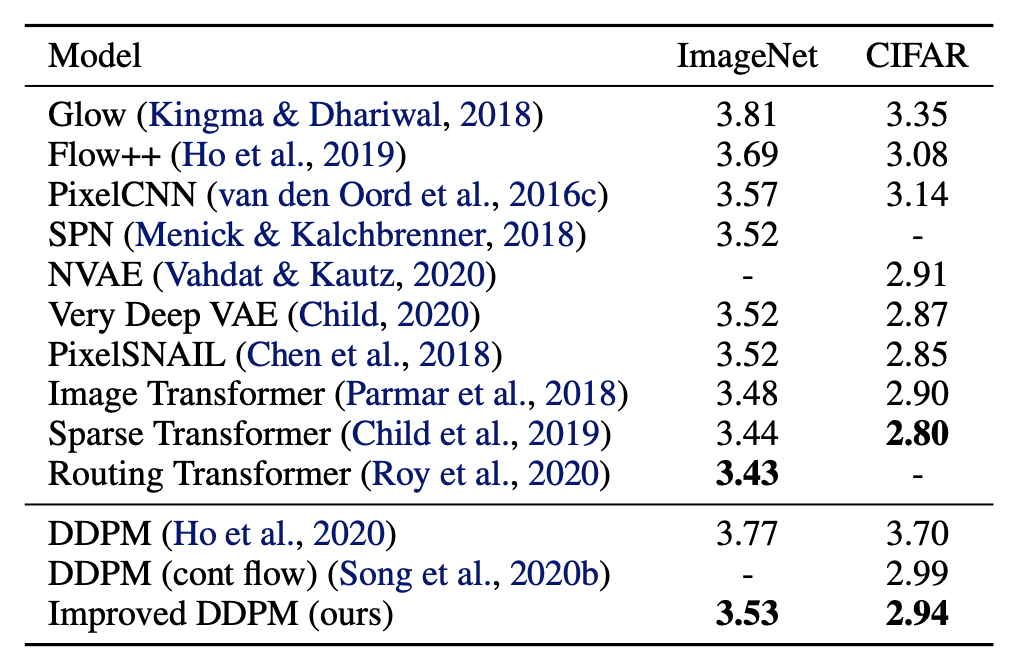
\includegraphics[width=5in]{\images/DiffNLL}}

\slide{Rewriting the VLB}

For a progressive VAE with layers $z_0,\ldots,z_L$ where $z_0 = y$ the VLB is

{\huge
\begin{eqnarray*}
- \ln p_{\gen}(z_0) & \leq & E_\enc\; -\ln \frac{p_\gen(z_L,\ldots,z_0)}{p_\enc(z_1,\ldots,z_L|z_0)}
\\
\\
\\
& = & E_\enc -\ln p_\pri(z_L) - \sum_{\ell } \frac{\ln p_\dec(z_{\ell-1}|z_\ell)}{\ln p_\enc(z_\ell|z_{\ell-1})}
\end{eqnarray*}
}

\slide{Rewriting the VLB}

{\huge
\begin{eqnarray*}
- \ln p_{\gen}(z_0) & \leq & E_\enc -\ln p_\pri(z_L) - \sum_{\ell } \ln \frac{p_\dec(z_{\ell-1}|z_\ell)}{p_\enc(z_\ell|z_{\ell-1})} \\
\\
& = & E_\enc -\ln p_\pri(z_L) - \sum_{\ell } \ln \frac{p_\dec(z_{\ell-1}|z_\ell)}{p_\enc(z_\ell|z_{\ell-1},z_0)} \\
\\
& = & E_\enc -\ln p_\pri(z_L) - \sum_{\ell } \ln \frac{p_\dec(z_{\ell-1}|z_\ell)p(z_{\ell-1}|z_0)}{p_\enc(z_\ell,z_{\ell-1}|z_0)} \\
\\
& = & E_\enc -\ln p_\pri(z_L) - \sum_{\ell } \ln \frac{p_\dec(z_{\ell-1}|z_\ell)p_\enc(z_{\ell-1}|z_0)}{p_\enc(z_{\ell-1}|z_\ell,z_0)p_\enc(z_\ell|z_0)}
\end{eqnarray*}
}

\slide{Rewriting the VLB}

{\huge
\begin{eqnarray*}
- \ln p_\gen(z_0) & \leq & E_\enc -\ln p_\pri(z_L) - \sum_{\ell } \ln \frac{p_\dec(z_{\ell-1}|z_\ell)}{p_\enc(z_{\ell-1}|z_\ell,z_0)}
- \ln \frac{p_\dec(z_{\ell-1}|z_0)}{p_\enc(z_\ell|z_0)} \\
\\
& = & E_\enc -\ln \frac{p_\pri(z_L)}{p_\enc(z_L|z_0)} - \sum_{\color{red} \ell \geq 2} \ln \frac{p_\dec(z_{\ell-1}|z_\ell)}{p_\enc(z_{\ell-1}|z_\ell,z_0)} - \ln p_\dec(z_0|z_1) \\
\\
\\
& = & E_\enc \left\{\begin{array}{l}KL(p_\enc(z_L|z_0),p_\pri(z_L)) \\
\\
+ \sum_{\ell \geq 2} KL(p_\enc(z_{\ell-1}|z_\ell,z_0),p_\dec(z_{\ell-1}|z_\ell)) \\
\\
- \ln p_\dec(z_0|z_1) \end{array} \right.
\end{eqnarray*}
}


\slide{Rewriting the VLB}

{\huge
  \begin{eqnarray*}
    - \ln p_\gen(z_0) & \leq & E_\enc \left\{\begin{array}{l}KL(p_\enc(z_L|z_0),p_\pri(z_L)) \\
\\
+ \sum_{\ell \geq 2} KL(p_\enc(z_{\ell-1}|z_\ell,z_0),p_\dec(z_{\ell-1}|z_\ell)) \\
\\
- \ln p_\dec(z_0|z_1) \end{array} \right.
\end{eqnarray*}
}

All of the KL-divergences can be computed analytically from Gaussians.  This reduces the variance in estimating the bound.

\vfill
Nichol and Dhariwal compute $- \ln p_\dec(z_0|z_1)$ by treating each image channel as a discrete set of 256 values and computing the probability that a draw from
the computed Gaussian rounds to the actual discrete value.

\slide{Optimizing Per-Channel Decoder Variances}

We now introduce a decoder network $\tilde{\sigma}_\Psi(z_\ell,\ell) \in R^d$ to give the decoder noise level.

\vfill
$$\dec(z_\ell,\ell) = \frac{1}{\sqrt{1-\sigma_\ell^2}}\left(z_\ell - \sigma_\ell\; \epsilon(z_\ell,\ell)\right)\; +\; \tilde{\sigma}_\Psi(z_\ell,\ell)\odot\delta\;\;\;\;\delta \sim {\cal N}(0,I)$$

\vfill
The decoder noise network $\tilde{\sigma}_\Psi(z_\ell,,\ell) \in R^d$ is trained with the VLB objective.

\vfill
This improves the value of the VLB.

\slide{Optimizing Per-Channel Decoder Variances}

$$\dec(z_\ell,\ell) = \frac{1}{\sqrt{1-\sigma_\ell^2}}\left(z_\ell - \sigma_\ell\; \epsilon(z_\ell,\ell)\right)\; +\; \tilde{\sigma}_\Psi(z_\ell,\ell)\odot\delta\;\;\;\;\delta \sim {\cal N}(0,I)$$

\vfill
One can interpret $\tilde{\sigma}(z_\ell,\ell)[i]$ is a level of uncertainty in the decoder value $\epsilon(z_\ell,\ell)[i]$.

\vfill
The more uncertainty the model has in $\epsilon(z_\ell,\ell)[i]$ the more guidance should be used in adjusting it.


\slidetwo{Diffusion Models Beat GANs on Image Synthesis}{Dharwali and Nichol, May 2021}

This paper introduces guided diffusion as a way of handling class-conditional diffusion models.

\vfill
\centerline{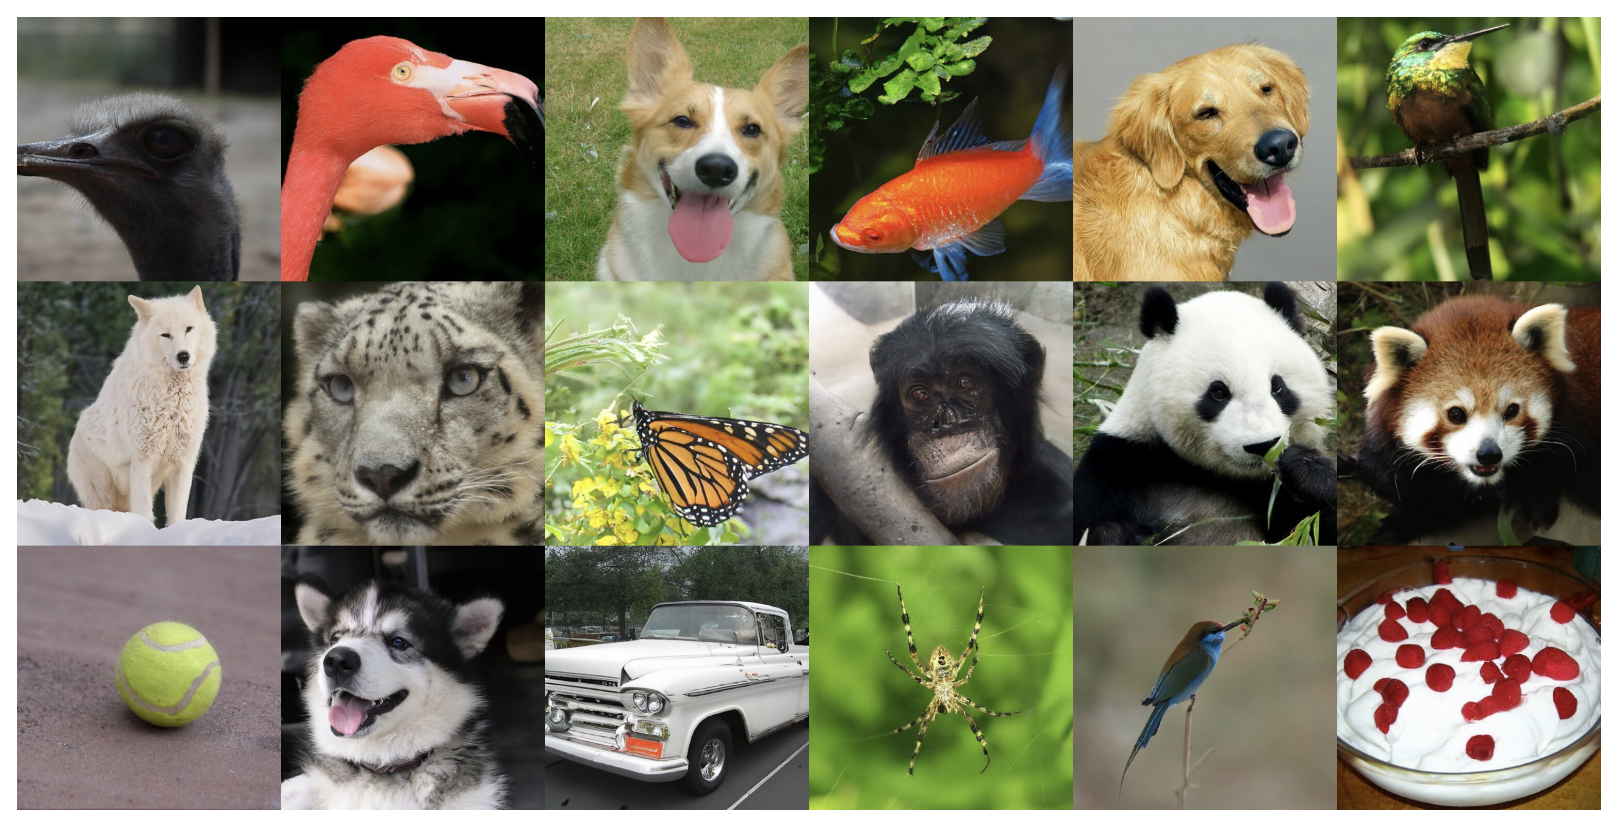
\includegraphics[width = 6in]{\images/DiffGAN}}

\vfill
Guided diffusion is used in DALLE-2.

\slide{Class-Conditional Image Generation}

We assume training data consisting of $(x,y)$ pairs and we want to generate from the distribution $P(y|x)$.  For example class-conditional image generation.

\vfill
Previous approaches, such as StyleGAN, have trained a model (a GAN) for each class.

\vfill
Here we will train a single model which takes the class label as input.

\vfill
It seems that this can be made to work for VAEs but not for GANS without an auto-encoder component.

\slide{Conditional Diffusion Models}

An obvious approach is to draw a pair $(x,y)$ and pass the conditioning information $x$ to the image genertor.

\vfill
It is a weakness of GANs that we need a separate model for each $x$.

\vfill
It seems to be a weakness of diffusion models that this natural approach to conditioning fails.

\slide{Classifier Guidance}
We assume a distribution on pairs $(x,y)$.

\vfill
We also assume {\bf a classifier} $P(x|y)$.  For example $x$ might be the ImageNET label for image $y$.

\vfill
We will generate an image by using $P(x|y)$ to ``guide'' generation from the unconditional model $\epsilon(z_\ell,\ell)$.

\vfill
Guidance will be based on the score-mathching interpretation of diffusion models where
$\epsilon(z_\ell,\ell)$ is interpreted as $- \nabla_z \ln p(z)$.

\slide{Class-Conditional Generation}

{\huge
\begin{eqnarray*}
  z_{\ell-1} & = & \frac{1}{\sqrt{1-\sigma_\ell^2}}\left(z_\ell - \sigma_\ell\; \epsilon(z_\ell,\ell)\right)\; +\; \tilde{\sigma}_\ell\odot\delta
\end{eqnarray*}
}

\vfill
Score-matching interprets $\epsilon(z_\ell,\ell)$ as $- \nabla_z \ln p(z)$.

\vfill
$$p(z|x) = \frac{P(z)P(x|z)}{P(x)} \propto p(z)P(x|z)$$

\vfill
We want a step in direction $\nabla_z\;\ln p(z)P(x|z)$. They use

{\huge
\begin{eqnarray*}
  \dec(z_\ell,\ell) & = & \frac{1}{\sqrt{1-\sigma_\ell^2}}\left(z_\ell - \sigma_\ell\; \epsilon(z_\ell,\ell)\right) \; +\; \tilde{\sigma}_\ell\odot\delta\; + {\color{red} s\tilde{\sigma}\odot\nabla_{z} \ln P(x|z)}
\end{eqnarray*}
}

\slide{Classifier Guidance}

{\huge
\begin{eqnarray*}
  \dec(z_\ell,\ell) & = & \frac{1}{\sqrt{1-\sigma_\ell^2}}\left(z_\ell - \sigma_\ell\; \epsilon(z_\ell,\ell)\right) \; +\; \tilde{\sigma}_\ell\odot\delta\; + {\color{red} s}\tilde{\sigma}\odot\nabla_{z} \ln P(x|z)
\end{eqnarray*}
}

Here $s$ is called the scale of the guidance.

\vfill
Empirically it was found that $s > 1$ is needed to get good class-specificity of the generated image.

\vfill
However, increasing $s$ decreases diversity so we have a diversity/quality trade off.

\slide{Other Improvements}

Various architectural choices in the U-Net were optimized based on FID score (not NLL).

\vfill
These improvements are used in DALLE-2.


\slidetwo{Classifier-Free Diffusion Guidance}
{Ho and Salimans, December 2021 (NeurIPS workshop)}

Classification diffusion guidance uses a classifion model $P(x|y)$.

\vfill
This paper introduces ``classifier-free'' diffusion guidance.

\vfill
Classifier-free diffusion guidance is used in DALLE-2.

\slide{Classifier-Free Diffusion Guidance}

5\% of the time we set $x = \emptyset$ where $\emptyset$ is a fixed value unrelated to the image.

\vfill
The decoder then uses

$$\tilde{\epsilon}(z_\ell,\ell,x) = s\epsilon(z_\ell,\ell,x) - (s-1)\epsilon(z_\ell,\ell,\emptyset)$$

\vfill
where $s \geq 1$ controls the relative weight of the two terms.

\vfill
DALLE-2 incorporates the channel-level uncertainties $\tilde{\sigma}$ as weights on classifier-free diffusion guidance provided by CLIP.

\slidetwo{Image Super-Resolution via Iterative Refinement}{Saharia, Ho et al., April 2021}

They construct a super-resolution diffusion model as conditional model for pairs for pairs $(x,y)$ with $x$ is a downsampling of $y$.

\vfill
\centerline{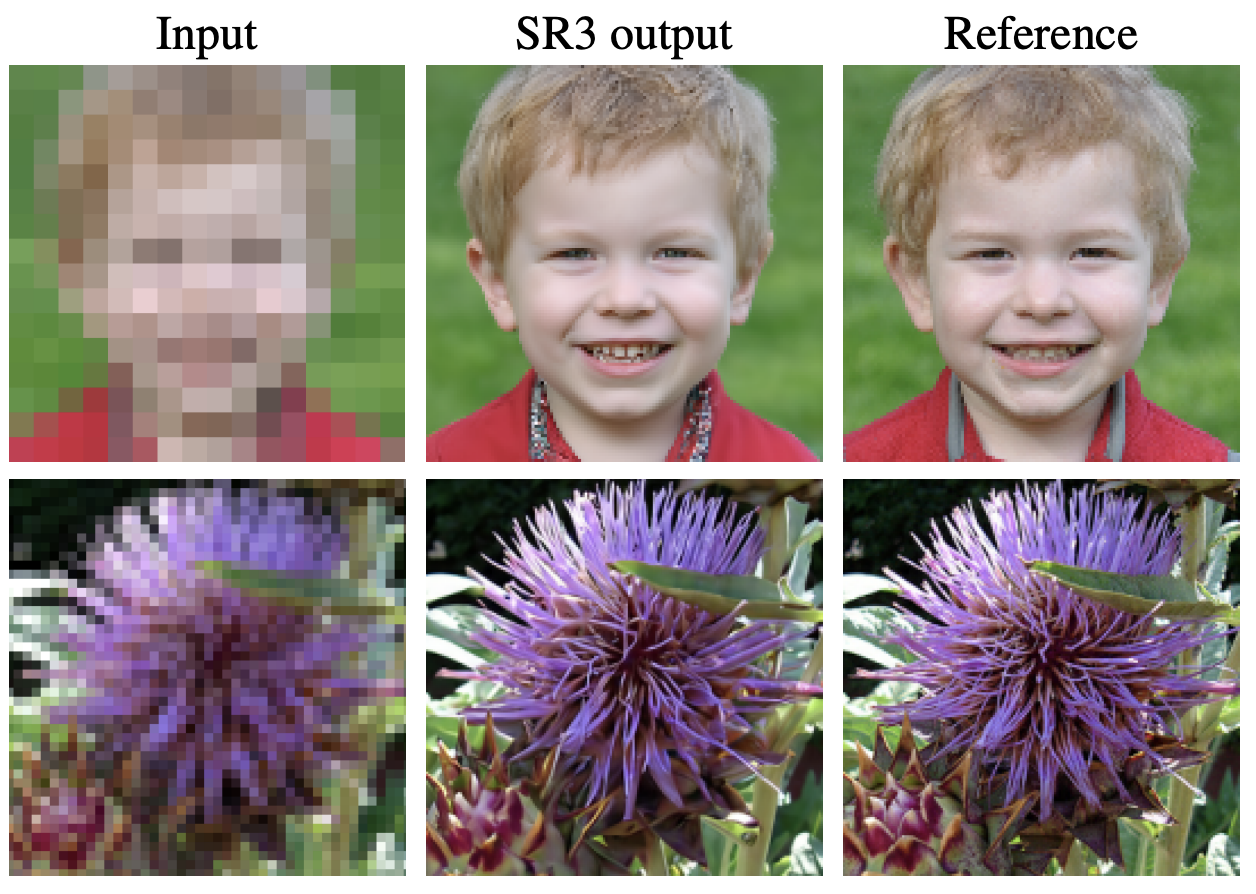
\includegraphics[width = 4 in]{\images/DiffUp1}}

\slidetwo{Cascaded Diffusion Models ...}{Ho, Saharia et al, May 2021}

A series of super-resolution diffusion models each conditioned on a class label.

\centerline{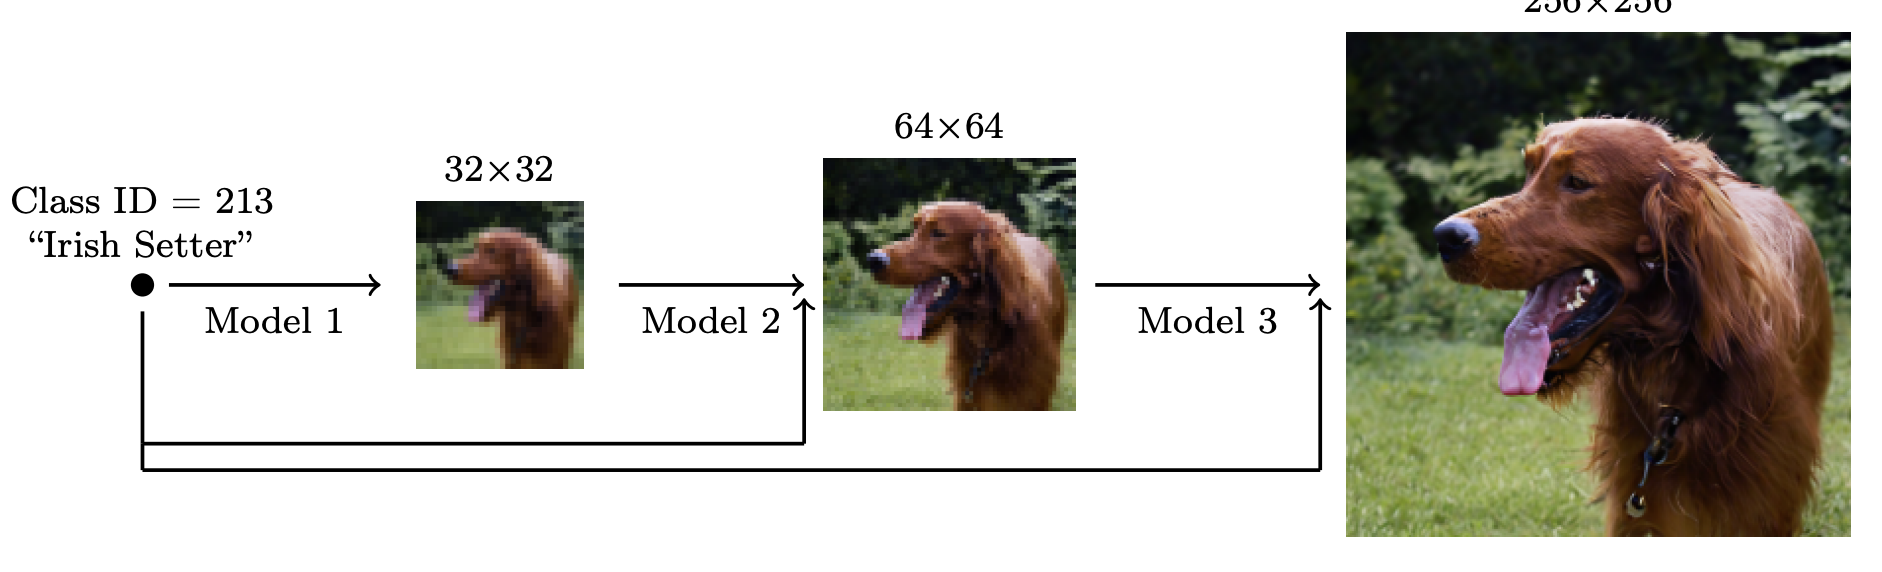
\includegraphics[width = 8 in]{\images/DiffUp2}}

\vfill
This architecture is used in DALLE-2.

\slide{CLIP Does Contrastive Coding}

\centerline{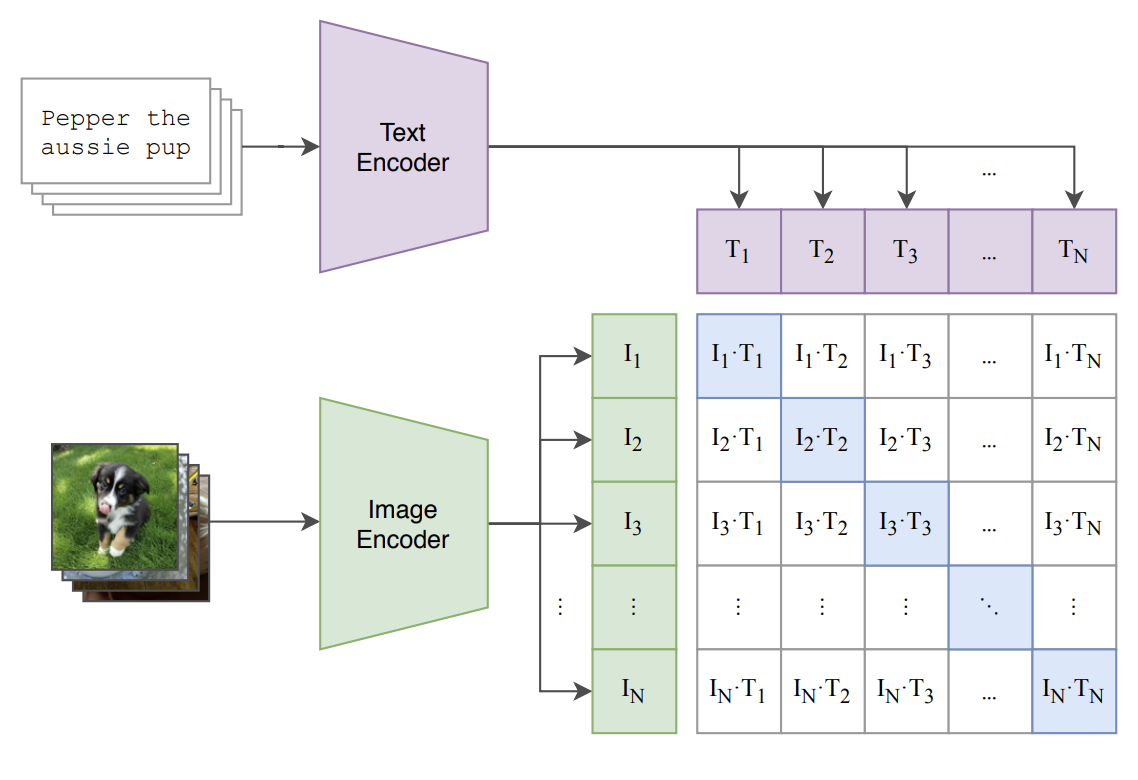
\includegraphics[height= 4in]{\images/CLIPTraining}}

\vfill
CLIP is used in DALLE-2 and in DALLE-2's predicessor GLIDE.

\slidetwo{GLIDE: Towards Photorealistic Image Generation ...}
         {Nichol, Dhariwal, Ramesh, et al., December 2021}

GLIDE compares two forms of diffusion guidance.

\vfill
\begin{itemize}
\item[(a)] Classifier-free guidance based on comparing conditioned and unconditioned decoding directions.

\vfill
\item[(b)] Classifer guidance based on CLIP.
\end{itemize}

\slide{Classifier-free (self-guided) GLIDE}

$$\tilde{\epsilon}(z_\ell,\ell,x) = s\epsilon(z_\ell,\ell,x) - (s-1)\epsilon(z_\ell,\ell,\emptyset)$$

\vfill
Classifier-free GLIDE does not use CLIP.

\vfill
The classifier-free guidance differs from the original version in that here we are conditioning on text
rather than as Imagenet labels.

\vfill
The text is transformed to a feature vector by a transformer before being fed to the decoder.

\slide{CLIP-guided GLIDE}

Let $C_I(y)$ be the CLIP vector for image $y$ and let $C_T(x)$ be the CLIP vector for text $x$.

{\huge
\begin{eqnarray*}
z_{\ell-1}  & = & \frac{1}{\sqrt{1-\sigma_\ell^2}}\left(z_\ell - \sigma_\ell\; \epsilon(z_\ell,\ell) + {\color{red} s \tilde{\sigma}\odot\nabla_{z} C_T(x)^\top C_I(z)}\right)\; +\; \tilde{\sigma}_\ell\odot\delta
\end{eqnarray*}
}

\vfill
Here CLIP is re-trained to handle noised images.

\slide{Upsamling}

Both GLIDE versions use diffusion upsampling to go from $64 \times 64$ to $256 \times 256$.

\vfill
The GLIDE paper concludes that the classifer-free model taking raw text as input is superior to the CLIP-guided model.

\slidetwo{DALL$\cdot$E-2}{Ramesh, Nichol, Dhariwal, et al., March 2022}

\centerline{\hfill 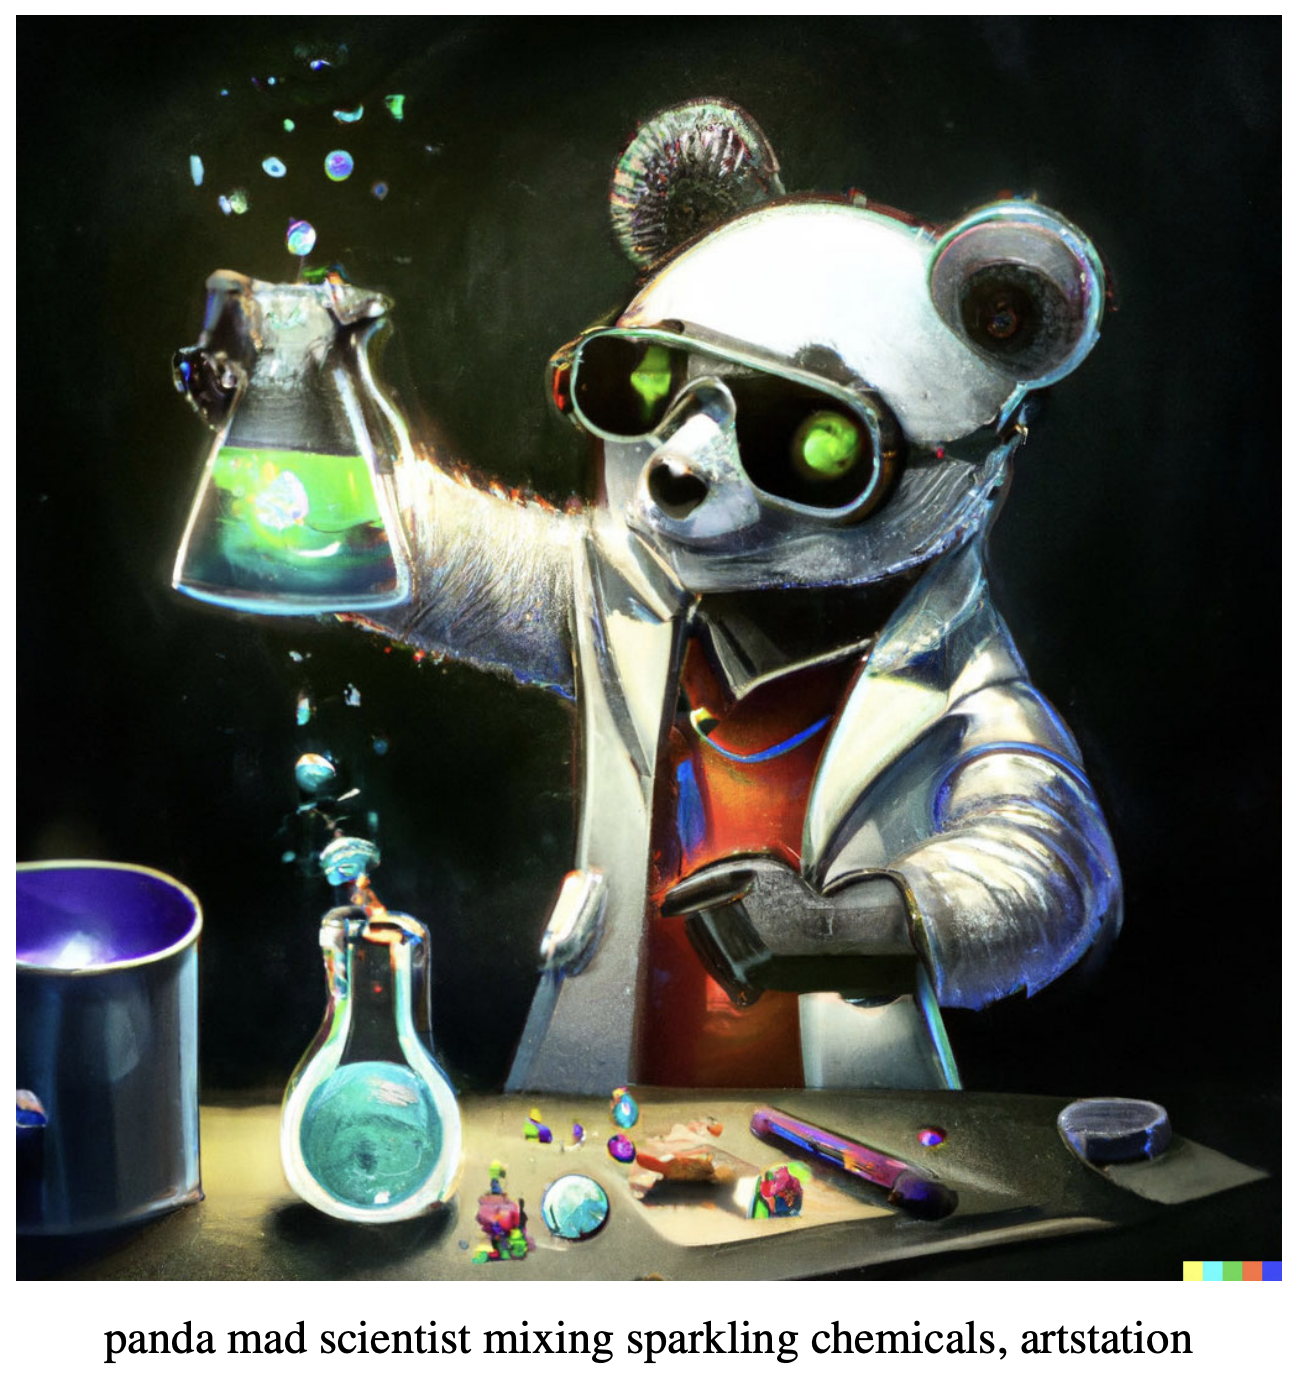
\includegraphics[width = 3.5 in]{\images/DALLEpanda} \hfill \includegraphics[width = 3in]{\images/DALLE2}}

CLIP-guided DALLE-2 is similar in quality to self-guided GLIDE but is more diverse.

\slide{DALL$\cdot$E-2}

\vfill
\centerline{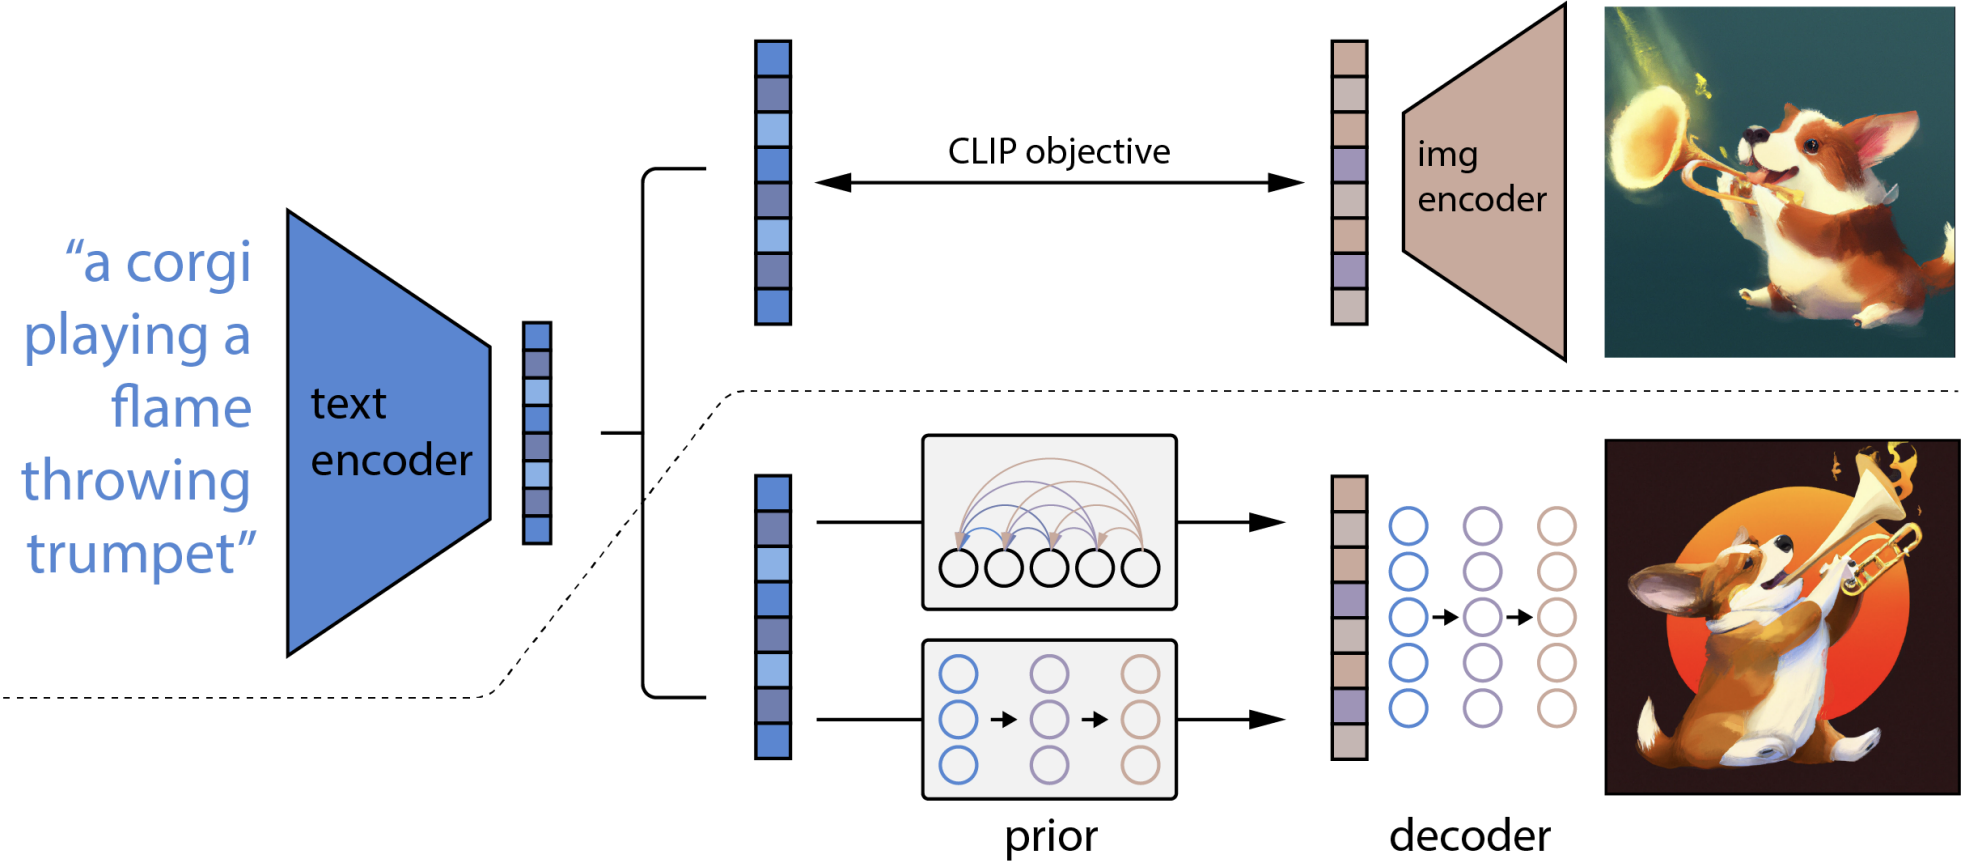
\includegraphics[width = 8in]{\images/DALLE2a}}

This figure is misleaning.  The lines in the figure do not correspond to the actual data paths of DALLE-2.

\slide{A Conditional Image Auto-Encoder}

\centerline{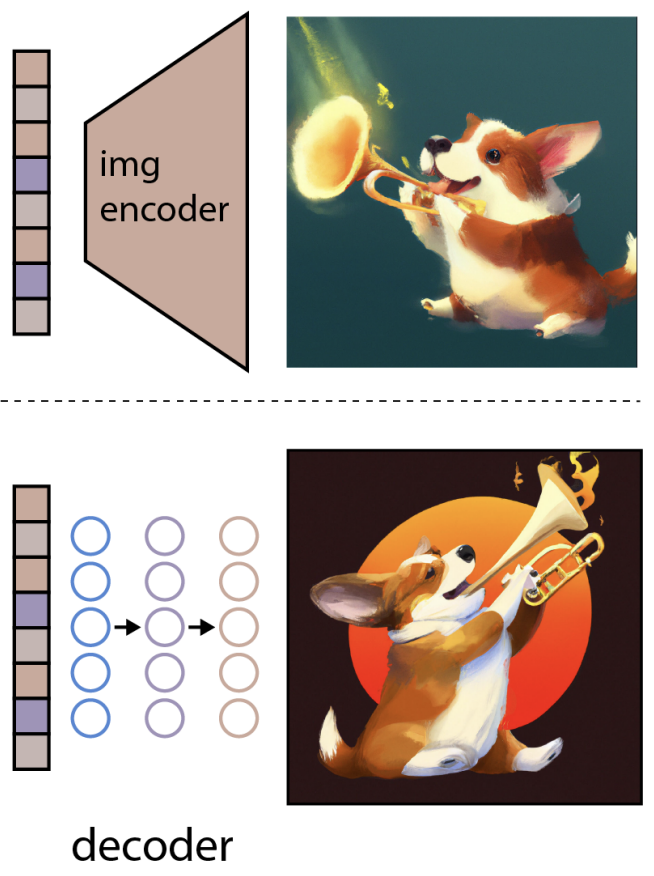
\includegraphics[height = 2.5in]{\images/DiffDALLE}}

\vfill
Let $C_I(y)$ denote the CLIP embedding of image $y$.

\vfill
$C_I(y)$ is the encoder of an auto-encoder for $y$ given $x$.

\vfill
$P(C_I(y)|x)$ is the optimal prior for this auto-encoder.

\vfill
$P(y|C_I(y),x)$ is the optimal decoder.

\vfill
In DALLE-2 the prior and the decoder both see the text $x$.

\slide{Putting it all Together}

We are given text $x$.

\vfill
Draw $\hat{C}$ from the prior $P(C_I(y)|x)$

\vfill
Do diffusion decoding with two upsampling models:

\vfill
\begin{quotation}
compute $\tilde{z}_{\ell-1}$ using $\hat{\epsilon} = s\epsilon(z_\ell,\ell,x) - (s-1)\epsilon(z_\ell,\ell,\emptyset)$
\vfill
$z_{\ell-1} = \hat{z}_{\ell-1} + s'\tilde{\sigma}\odot\nabla_z\;\hat{C}^\top C_I(z)$
\end{quotation}

\slide{The Prior}

They experiment with two priors $P(C_I(y)|x)$.

\vfill
An autoregressive model and a conditional diffusion model.

\vfill
They say both priors use self-guidance.

\slide{The Autoregressive Prior}

First do PCA on the distibution of vectors $C_I(y)$ to reduce their dimensionality from 1024 to 319.

\vfill
Sort the eigenvectors in decreasing order of eigenvalue.

\vfill
Quantize each of 319 values into 1024 discrete buckets.

\vfill
We train a transformer to take the vector $C_T(x)$ followed by the string $x$
and to predict a string of 319 symbols with a vocabulary of size 1024 which can be converted back into the vector $\hat{C}$.

\slide{The Diffusion Prior}

\centerline{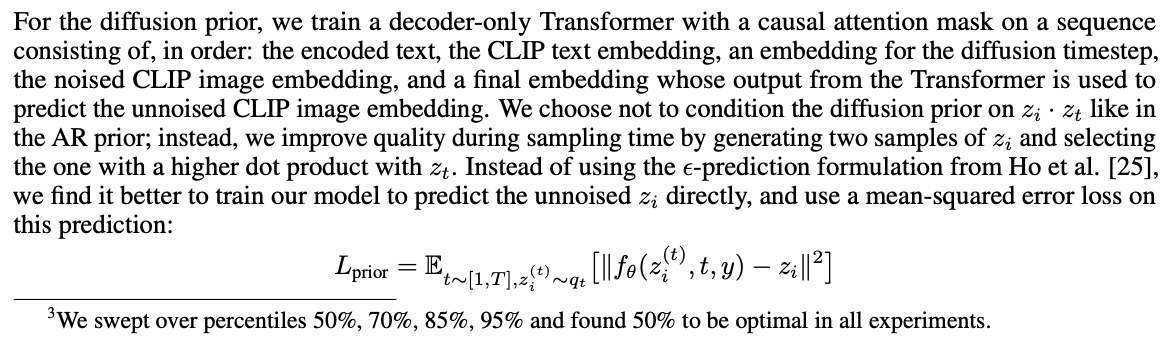
\includegraphics[width = 9in]{\images/DiffPrior}}

\vfill
\vfill
What?

\slide{Progressive VAEs}

Diffusion models are a special case of progressive VAEs.

\vfill
A progressive VAE has layers of latent variables $z_1,\dots,z_{L}$.

\vfill
It is not clear whether diffusion models are the best way to do this.

\vfill
It could be that the important idea is simply having large $L$ with
$I(z_0,z_\ell)$ going from $H(z_0)$ to 0 as $\ell$ goes from $0$ to $L$.


\slide{END}
}
\end{document}

